\documentclass[12pt, oneside]{article}

% Language setting
% Replace `english' with e.g. `spanish' to change the document language
\usepackage[english]{babel}

% Set page size and margins
% Replace `letterpaper' with `a4paper' for UK/EU standard size
\usepackage[letterpaper,top=2cm,bottom=2cm,left=3cm,right=3cm,marginparwidth=1.75cm]{geometry}

% Useful packages
\usepackage{amsmath}
\usepackage{graphicx}
\usepackage[colorlinks=true, allcolors=blue]{hyperref}
\usepackage{graphicx} % Required for inserting images
\usepackage{cite}
\usepackage{amsmath,amssymb,amsfonts}
\usepackage{algorithmic}
\usepackage{graphicx}
\usepackage{textcomp}
\usepackage{xcolor}
\usepackage{csquotes}
\usepackage{placeins}
\usepackage{etoolbox}
\usepackage{IEEEtrantools}


\begin{document}

\begin{titlepage}
    \begin{center}
        \vspace*{1cm}
        {\huges
        \center{\huge{\textbf{Dissertation Project Research Proposal}}}}
         \\
         \vspace{0.3cm}
         \large{Self-organised Resource Sharing for Decentralised Multi Agents on 2D plane Based on STDMA}
         \vspace{0.5cm}
        \\
        {\large By}
        \\
        \vspace{0.5cm}
        \textbf{Runze Yuan}
   		\vspace{1.5cm}
        \\
        \vspace{0.25cm}
       
\includegraphics[scale=0.6]{logos/bristolcrest_colour.pdf}
        \hspace{5mm}
        
\includegraphics[scale=0.35]{logos/UWE_insignia.png}

        \vspace{10mm}
        {\large Department of Engineering Mathematics\\
        \textsc{University of Bristol}}
        \\
        \&
        \\
        {\large Department of Engineering Design and Mathematics\\
        \textsc{University of the West of England}}\\

        \vspace{0.8cm}
 
        \vspace{0.8cm}
        \today
        
    \end{center}
    
\end{titlepage}

\tableofcontents
\pagebreak

\section{Aims and Objectives}
\subsection{Aims}
Based on the self-organised channel resource allocation principle of the STDMA(Self-organised Time Division Multiple Access) \cite{STDMA} communication protocol, develop a method for agents to achieve collision-free moving on a 2D plane, make it self-organised, decentralised and scalable. 

\subsection{Objectives}
\label{Objectives}
\begin{itemize}
    \item Develop a multi agent communication scenario with STDMA in ROS2. In this scenario, multiple identical agents will share the same channel and all agents have both receiving and transmitting capabilities. The goal is to enable agents to autonomously organise/join the communication process after start up.
    % 使用ROS2与其node实现多agent的通信场景模拟。在此场景中,多个相同的agent将共享同一个信道,且agent都具有收发功能,agents应当能自动地组织/在开机后加入通信过程。目标是使agent能够在开机后自主地组织/加入通信过程。
    \item On the basis above, a simple grid world is implemented: a 2D map composed of grids, each grid representing a part of space. Agents would move from one grid to another on the map.
    % 在上述基础上实现简单的二维地图导航情景:一张由若干网格组成的二维地图,每一个网格代表空间的一部分。agent的运动就是在地图中从一个格子移动到另一个格子。格子的形状不仅限于四边形[],这里需要后续进一步研究确定。
    \item Using the principle of STDMA \cite{STDMA} to implement simple decentralized conflict-free space(which is a kind of resource) sharing and simulate implementation in the above scenario.
    % 用STDMA的原理实现简单的去中心化无冲突空间(其也是某种资源)分享,并在上述场景中模拟实现。
    \item STDMA is designed for 1D resource sharing (slots in time frames), and directly applying STDMA for 2D space sharing will definitely lead to some deadlock and inefficient scenarios\cite{MAPF_Deadlock_Explain1,MAPF_Deadlock_Explain2}. Determine the cause of this problem by observing the experiment, and make corresponding improvements to this problem. 
    % 直接套用STDMA一定会导致某种死锁和低效的场景发生[]。通过实验模拟定位此类场景发生的原因并进行改进,设计一些资源分享中的规则,并提升算法的表现。
    \item Use appropriate performance metrics (makespan, sum of cost, and agent capacity when algorithm running in widely used benchmark maps\cite{MAPF_Deadlock_Explain2}) to evaluate the advantages and disadvantages of algorithm performance. 
    % 选取合适的性能指标,评判算法性能的优劣。
\end{itemize}


\section{Motivation}

The motivation of this project is to answer a question inspired by \cite{Paper_From_Supervisor}. Which is:

\label{Question}

\begin{displayquote}
\textbf{What will happen if use STDMA for 2D resource sharing?}
\end{displayquote}

The detailed explanation of the motivation is as follows.

\subsection{Why STDMA?}
\label{Why STDMA}
\textbf{What is STDMA?} The \textit{Self-organised Time Divided Multi Access} (STDMA) is an channel access technique for communication. It is based on a set of policies dictating how agents ought to apply for slots in repeating frames, as elaborated in Section \ref{STDMA_Explained}.

 \vspace{0.4cm}

The reason for using STDMA is its \textbf{characteristics}\cite{STDMA_characteristic}:
\begin{enumerate}
    \item \textbf{Deterministic}: Agents arrange their data transmission based on a determined timetable.
    \item \textbf{Decentralised}: Agents listen to the channel first, then find free slots in the timetable for themselves to use.
\end{enumerate}

These characteristics could be useful for multiple agents to achieve collision-free (use free slots only), self-organised (find slots on its own) resource sharing.

There are also two \textbf{reasons that making this challenging}:
\begin{enumerate}
    \item \textbf{Dimensional Difference}: STDMA is designed for sharing discrete time slots(1D), and cannot be directly applied to resource sharing in a 2D plane. Modification is needed for 2D space application.
    \item \textbf{Moving by Grids}: In the communication scenario, agents don't have destinations in the timetable, i.e., don't need to move to a specific slot in the table. But that's different for 2D space moving, where agents have their destinations and need to move grid by grid to reach their goals. Agents could easily be trapped in situations of inefficiency or even deadlock situations \cite{MAPF_Deadlock_Explain1,MAPF_Deadlock_Explain2}.
\end{enumerate}

These characteristics and challenges are making this topic interesting and need further experiment to investigate.

\subsection{Why 2D resource sharing?}

    2D resource sharing is a name for better understanding and is not the accurate name for this problem. This problem is actually a \textbf{\textit{Multi-Agent Path Finding}} (\textbf{MAPF})\cite{MAPF_Deadlock_Explain2} problem. 
    
    Here, the term "finding" could be somewhat confusing. In fact, he MAPF problem combines both \textbf{collision-free movement} of multiple agents and \textbf{path efficiency optimising}.

    Overall, the problem of \textit{Multi-Agent Path Finding} (MAPF) concerns \textbf{the movement of multiple agents in a grid world}.
    
    To easily get a better understanding of this problem, please refer to this \href{https://primalgrid.netlify.app/primal}{website} \footnotemark.\footnotetext{https://primalgrid.netlify.app/primal} The website presents the MAPF problems and their solutions through a simple and engaging animation (estimated time required: 1$\sim$2 min). For detailed explanation, please see Section \ref{MAPF_Review}.
    \\[8pt]
    \textbf{MAPF algorithms have broad prospects for use}.
    % 下面列出若干应用的分类 itemize
    \begin{itemize}
        \item \textbf{Warehouse Automation}: Pick-pack-and-ship system in Amazon warehouse (like Fig \ref{fig:Amazon Warehouse Robots}.) \cite{Amazon_Kiva}. Delivering items in sorting station\cite{Warehouse_Automation1,Warehouse_Automation2}.
        \item \textbf{Intersection Management}: Coordinate autonomous vehicle movement through intersections \cite{Intersection_Management}.
        \item \textbf{Robot Fleet}: Automating fleets of autonomous robots like forklift fleets.\cite{Fork_Fleet1,Fork_Fleet2}.  
        \item \textbf{Agents in video games and CGIs}: Flock simulating and animating\cite{Flocking_1,Flocking_2}.
        \item \textbf{Swarm Robots}: Controlling self-organised robot swarms\cite{Swarm_Robotics}.
        \item \textbf{...}
    \end{itemize}

\begin{figure}
    \centering
    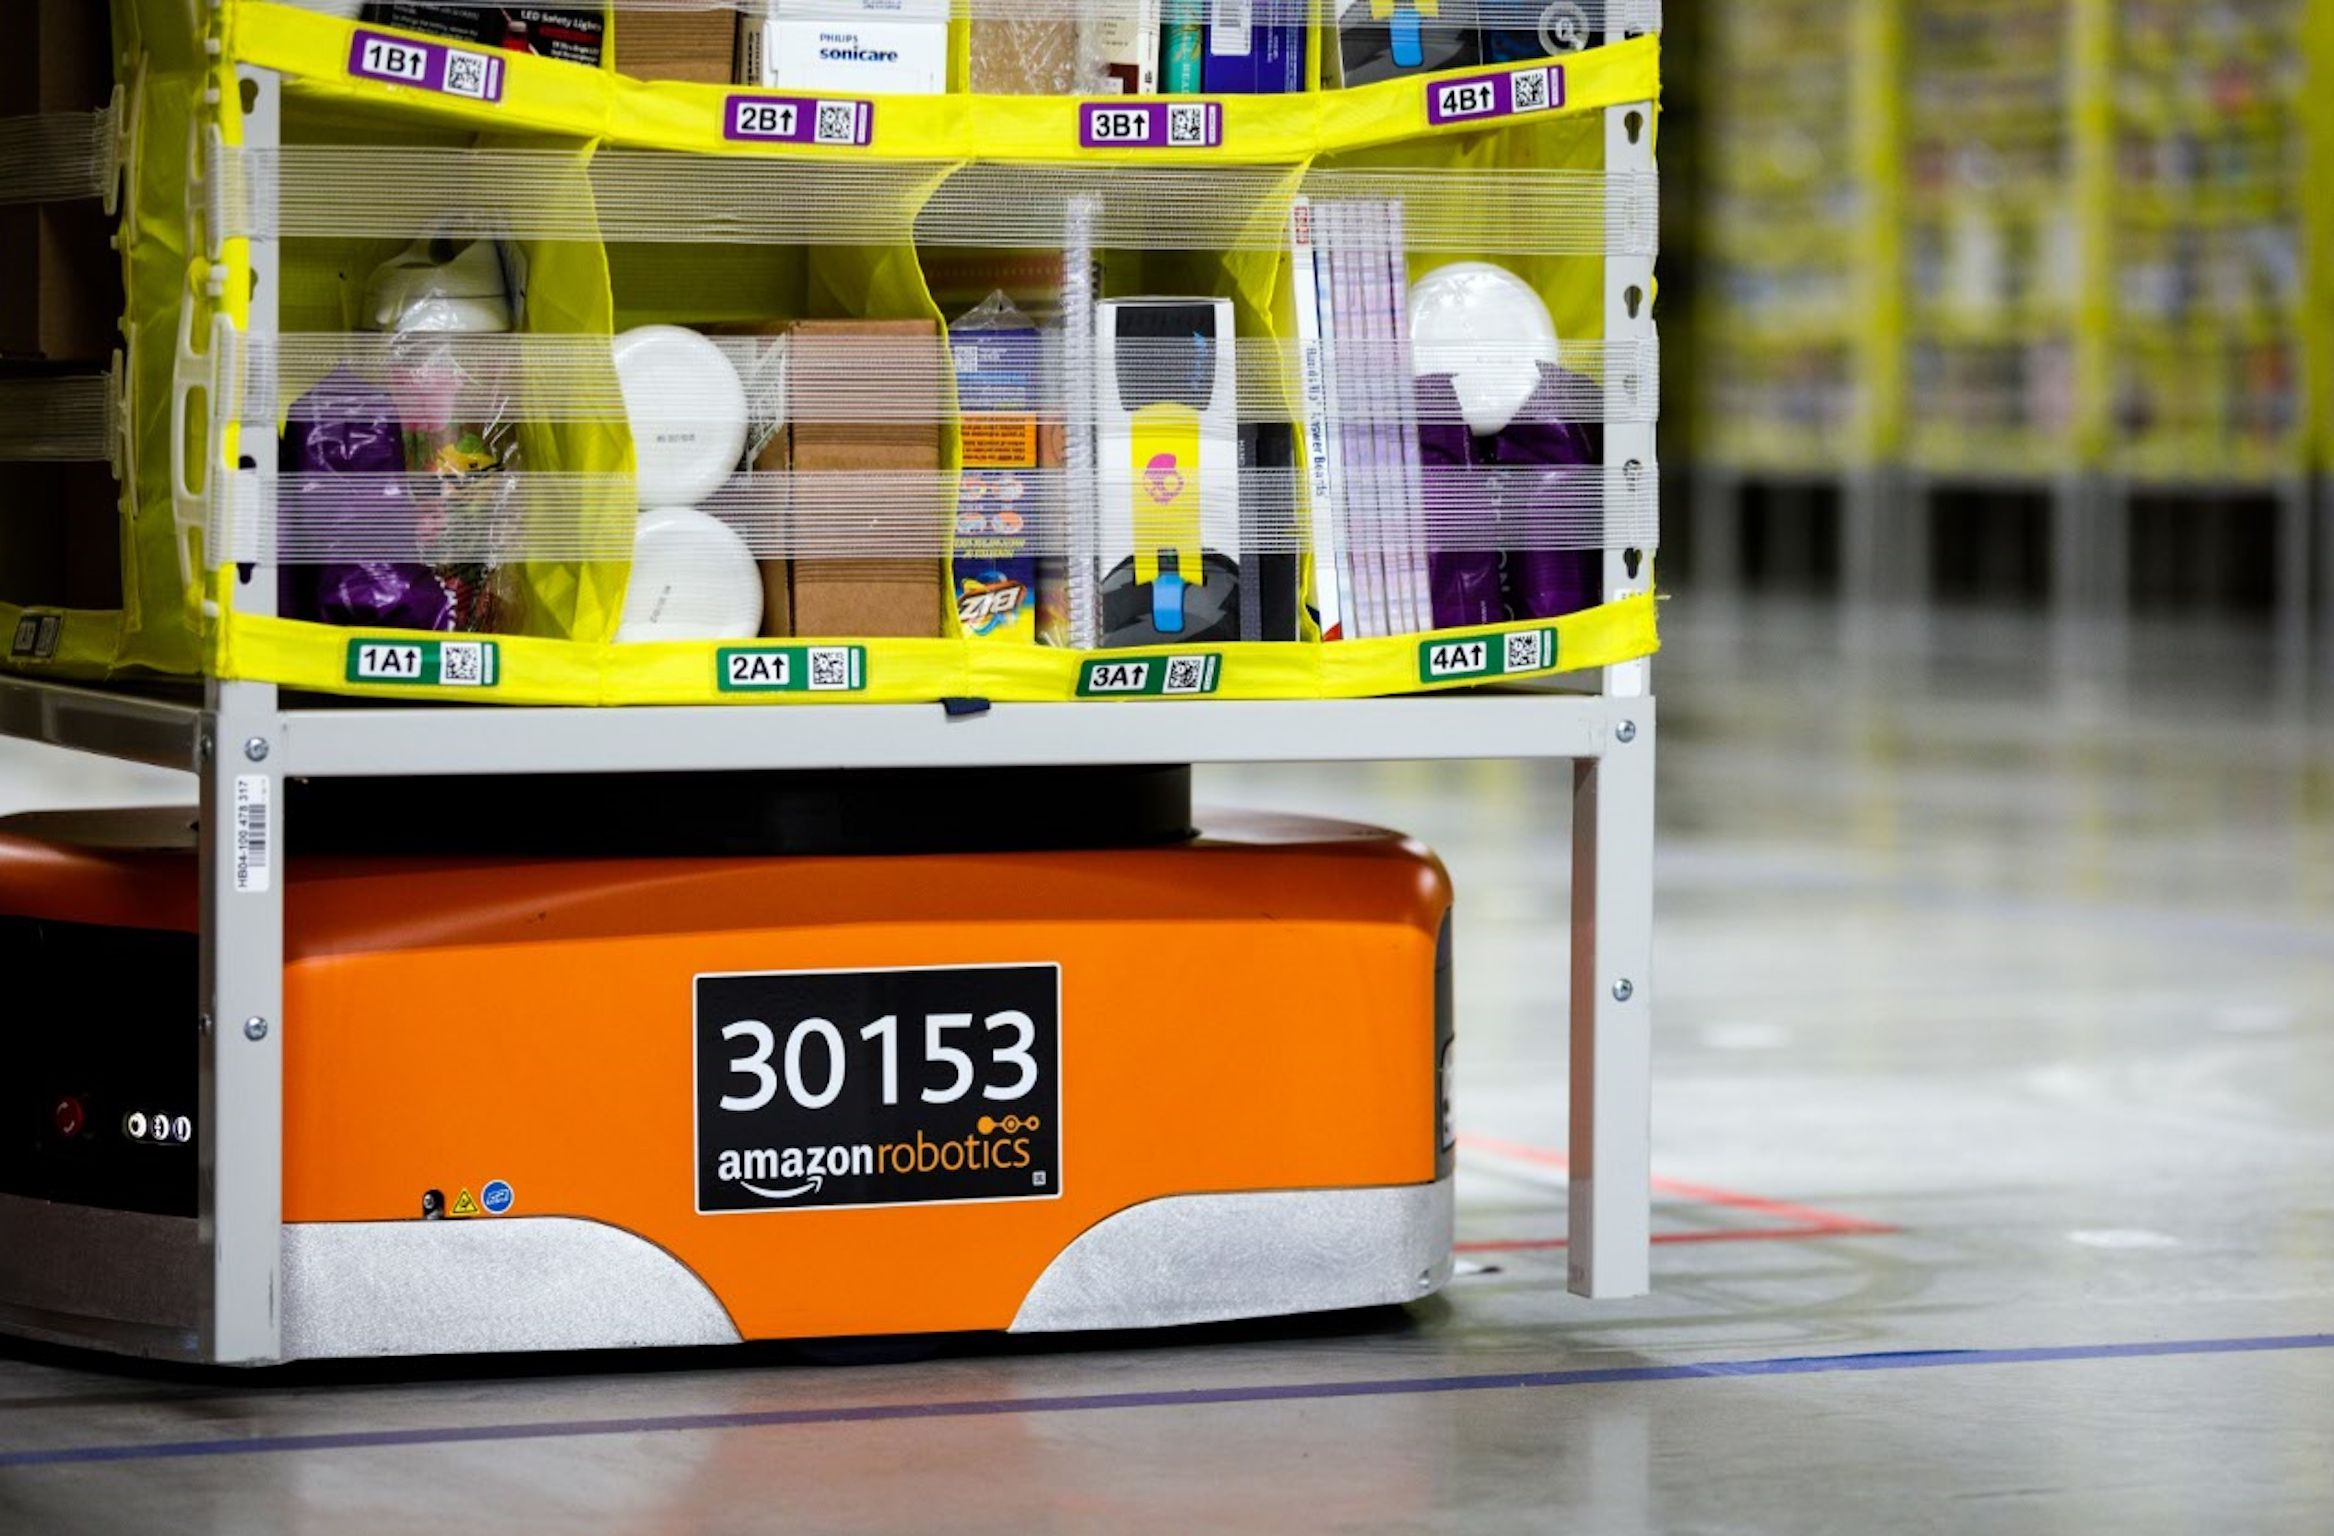
\includegraphics[width=0.6\linewidth]{Amazon_Warehouse.jpeg}
    \caption{Kiva system operating in Amazon warehouse.\footnotemark[1] }
    \label{fig:Amazon Warehouse Robots}
\end{figure}

\footnotetext{https://spectrum.ieee.org/interview-brad-porter-vp-of-robotics-at-amazon}

    
    %  说,总体来说,此种技术的应用是非常广泛的。且在工业4.0和柔性制造的环境下,有更好的应用前景.11,17,5

    In general, the application of this algorithm is very broad. Furthermore, in the context of Industry 4.0 and flexible manufacturing, it has even better prospects for application\cite{Industry_41,Industry_42,Industry_43}, as centralized control is gradually becoming inadequate to meet new production needs.


\section{Literature Review}
\label{LiteratureReview}

% 在此部分将会介绍STDMA协议的细节,并总结相关MAPF算法的发展。
This section will introduce the details of the STDMA\cite{STDMA} protocol and summarize the development of relevant MAPF algorithms.
\subsection{STDMA Explained}
\label{STDMA_Explained}


As previously mentioned in Section \ref{Why STDMA}, STDMA\cite{STDMA} allows multiple devices to share the same channel for communication without centralised control. The main assumption of this protocol is that all devices have synchronized clocks. In practice, this is achieved through GPS\cite{STDMA_2}.

\textbf{The core idea of STDMA can be summarized as follows}: Represent continuous time with repeated frames, each frame has several discrete slots. While devices are always listening to channel information, they look for free slots to occupy for their broadcasting their own data.



Devices using STDMA have \textbf{four phases}, which are arranged in chronological order as follows:

\begin{enumerate}
    \item \textbf{Initialisation}: Devices in this phase have not yet joined the network. The device listens to an entire frame and determines the current slot allocation.
    \item \textbf{Network Entry}:  Randomly choose an unallocated slot to broadcast their existence and reserve one slot for the next phase.
    \item \textbf{First Frame}: Use the slot reserved in the previous phase to reserve more slots for themselves. The number of reserved slots depends on the size of the data packet that the device needs to send.
    \item \textbf{Continuous Operation}: Use the previously reserved slot to work normally. If some slots are released or more slots are needed, reapply for slots.
\end{enumerate}

Although the above description omits some details (such as slot choosing methods, calculation of required number of slots, etc.), it is clear that \textbf{the core of STDMA is the strategy of finding and reserving unallocated slots}.

% 最后记得写一下STDMA的假设。
This protocol also has some limitations, such as: \textbf{(1)} Collision: In Network Entry phase, multiple devices may accidentally choose the same unallocated slot to broadcast their existence. \textbf{(2)} Capacity: When the slots are not enough, conflicts will inevitably occur.There are some studies \cite{STDMA_improv1,STDMA_improv2} that proposed improvements to the above limitations, but this is not the focus of this project.


\subsection{MAPF Algorithm Review}
\label{MAPF_Review}

The classical definition of the MAPF problem is: \textbf{Multiple agents moving step by step in an undirected graph in discrete time}\cite{MAPF_Deadlock_Explain1}.

\vspace{0.4cm}

For the MAPF problem with $n$ agents, its \textbf{inputs} are:

\begin{enumerate}
    \item \textbf{Environment}: The environment is represented as an undirected graph $G = (V, E)$, where vertices $V$ represent space in the environment and edges $E$ describe the connection of vertices.
    \item \textbf{Start}: The starting vertices of $n$ agents are represented with $s : [1, …, n] \rightarrow V_{s}$, which maps $n$ agents to the source vertices $V_{s}$.
    \item \textbf{Target}: The target vertices of $n$ agents are represented with $t : [1, …, n] \rightarrow V_{t}$, which maps $n$ agents to the source vertices $V_{t}$.
\end{enumerate}

For the MAPF problem with $n$ agents, it \textbf{requires}:

\begin{enumerate}
    \item \textbf{Single-agent Plan}: A sequence of actions. By executing this sequence of actions, an agent can reach the target from the start.
    \item \textbf{Solution}: A set of single-agent plans for all $n$ agents in the system. By executing the sequence of actions in this set simultaneously, all agents should be able to reach the destination from the starting point. A good solution should be both efficient and collision-free.
\end{enumerate}

% MAPF算法可以分为几种大类:传统的,启发式的,基于规则的,结合人工智能的。
The MAPF algorithm can be divided into \textbf{several categories: classical, heuristic, rule-based, and machine learning combined}. Among these categories, \textbf{the rule-based algorithms are the most relevant to this project}. However, I would also briefly introduce other types of algorithms.

\begin{itemize}
    \item \textbf{Classical}: The most popular classic MAPF algorithm is the \textit{Artificial Potential Field} (APF) algorithm, which put force fields around obstacles and goals to generate a force to guide the agents. APF methods does not guarantee collision-free and is prone to fall into local minima. There are still some research today dedicated to improving the performance of the APF algorithm, with a primary focus on optimizing the potential field function\cite{APF_improv2,APF_improv3,APF_improv4}.
    \item \textbf{Heuristic}: Heuristic algorithms mainly include A* and its variants (like  D* \cite{D*}). Heuristic algorithms mainly operate on the principle of searching for the optimal solution. Many research combine A* with other algorithms to achieve better performance and goes beyond the original A* \cite{A*_1,A*_2}.
    \item \textbf{ML Combined}: The machine learning algorithm mainly used in this field is reinforced learning, and usually combined with other non-RL techniques \cite{RL_1,RL_2,RL_3,RL_4}. 
    \item \textbf{Rule-based}: Most of the rule-based methods are based on the idea that each agent follows a set of identical local decision-making principles (which means it is decentralized) and usually improve algorithm performance by modifying the rules. Many of these algorithms are bio-inspired.
     \begin{itemize}
         \item \textbf{PSO}: The idea of \textit{Particle Swarm Optimization} is to simulate social behaviour of animals. \cite{PSO_1} improved the algorithm performance with swarm dynamics and designed a obstacle-avoidance algorithm for multi-UAV path finding. \cite{PSO_2} designed an algorithm for patrol robot and presented an interval update law for best position estimation, then applied an iterative procedure for obstacle avoiding.
         \item \textbf{GA}: \textit{Genetic Algorithm} is inspired by the process of natural selection that is popular for solving optimizing problems. \cite{GA_1} proposed an algorithm for UAV transmission which uses GA and RL to generate incentive rewards for agents. And \cite{GA_2} designed an algorithm for parking slot allocation with similar principle.
         \item \textbf{ACO}: \textit{Ant Colony Optimisation} is widely used for all questions that can be reduced to finding path to food through graphs. These algorithm usually are built with pheromone-based communication between agents. \cite{AGO_1} proposed an AGO-based algorithm for AGV that could do path finding and task allocating at the same time.  \cite{AGO_2} proposed an adaptive waypoints-repair method with reinitialisation mechanism integrated for multiple unmanned ground vehicle path planning.
         \item \textbf{PIO}: \textit{Pigeon-Inspired Optimisation} is inspired by the movement of pigeon flock going home. \cite{PIO_1} developed a path finding method for UAVs with PIO based on time stamp segmentation technique. \cite{PIO_2} improved the UAV path planning algorithm performance in plateau narrow area with cauchy mutant PIO algorithm.
         \item \textbf{GWO}: \textit{Grey Wolf Optimisation}\cite{GWO} is based on the leadership hierarchy and hunting mechanism of grey wolves. Agents are divided into four types to mimic the nature of grey wolf leadership hierarchy and applicable for problems with unknown possibility spaces.\cite{GWO_1} proposed a UAV path planning algorithm which is a hybrid of GWO and \textit{Whale Optimiser Algorithm} and is capable of avoiding dynamic obstacles. \cite{GWO_2} using GWO to solve multi-UAV path planning model with energy constraint, and improved the optimisation ability of GWO.
         \item \textbf{Push-and-Swap}: \textit{Push-and-Swap} algorithms \cite{Push_and_Swap} are based on two types of moves: push (move towards the goal) and swap (exchange position between two agents). It have many variants, and algorithms in this category are usually complete and fast. However, there is no guarantee that the solution given is optimal.  \cite{PaS_1} proposed a solution to pebble-motion on graphs with Push-and-Swap algorithm. \cite{PaS_2} built a MAPF algorithm with the principle of Push-and-Swap which provides theoretical completeness and optimality, but cannot deal with deadlocks on narrow passages.
     \end{itemize}
\end{itemize}

% 总体来说,MAPF问题有非常大量的不同解法,但所有解法都是在时间复杂度,完备性,最优解之间的平衡,还没有十全十美的算法出现。
In general, there are many different solutions to the MAPF problem, but \textbf{all algorithms are trade-offs between completeness, computational complexity, and optimality}. There is currently no perfect algorithm for this question.



\section{Impact Assessment}
% 本项目主要是对一种算法的模拟,因此其影响主要为潜在的影响。本项目的主旨在于通过回答一个问题来使读者对MAPF问题有更好的了解。
The main goal of this project is to help readers gain a better understanding of the MAPF problem by answering a question (see Section \ref{Question}), and the proposed algorithm is mainly based on simulation rather than practical system operation. Therefore, \textbf{the impacts of this project are mostly potential rather than immediate}.

 \vspace{0.5cm}

\textbf{Positives}:

\begin{itemize}
    \item Academical Impact: Help readers to get better understanding of MAPF problems and may provide inspiration to developers.
    \item Improve Production: MAPF could help agents to better navigate and accomplish tasks, improve efficiency, flexibility, and reduce costs.
    \item Increased Safety: Reduce the accidents and fatalities caused by human error.
\end{itemize}

\textbf{Neutral}:
 \begin{itemize}
     \item Energy Efficiency: MAPF algorithms helps the robot swarm to improve their energy efficiency by optimizing its route and reduce idle time. But there is also a risk of increased energy consumption due to the overuse of robots in production processes and accurately estimating the impact of this part is beyond my knowledge and ability.  
 \end{itemize}

\textbf{Negatives}:

\begin{itemize}
    \item Impact on Workforce: Implementation of MAPF algorithms could impact the workforce, potentially leading to job displacement or changes in job. Although it may also bring more R\&D personnel and technical personnel positions, considering the difference in the number of bases, the number of affected workers is overwhelming.
    \item Cultural Resistance: Application of MAPF algorithms could face resistance from cultural or social groups who value human labor and human-based decision making.
    \item Digital Security: Applications of MAPF algorithms (like AGVs) may introduce risks of cyber attack and private data leakage. 
\end{itemize}

\FloatBarrier

\section{Risk Register}

% 本项目从风险管理的角度可以这样描述: 我在有ROS2环境的具有普通笔记本电脑等级算力的电脑中,进行算法的模拟与优化。
From a risk management perspective, your project can be described as:
\begin{quote}
    \textbf{I} simulate and optimize \textbf{algorithms} in a \textbf{computer} with normal laptop-level computing power and \textbf{ROS2} environment.
\end{quote}


% 其中的可能风险由下表表示。对于其中的似然性和影响两栏,用1-4来衡量其等级,1代表最不可能/影响最小,4代表最可能/影响最大。
\textbf{The possible risks are represented by the table below}(Table \ref{RiskRegister}.). For the likelihood and impact columns, levels 1$\sim$4 are used for measuring, with 1 representing the least likely/least impact and 4 representing the most likely/most impact.



\begin{table}[]
\begin{tabular}{|l|l|l|l|}
\hline
Risk                      & Likelihood(A) & Impact(B) & Risk Score(A×B) \\ \hline
PC Malfunction            & 2             & 4         & 8               \\ \hline
Underestimated Complexity & 3             & 2         & 6               \\ \hline
ROS2 Capability           & 2             & 2         & 4               \\ \hline
Progress Loss             & 1             & 4         & 4               \\ \hline
\end{tabular}
\caption{Project Risk Register.}
\label{RiskRegister}

\end{table}



\textbf{PC Malfunction}: Due to some mysterious software malfunction, my computer has been performing very unstably. In fact, during the process of writing this proposal, I was forced to reinstall the operating system once. For this risk, I will try my best to solve it before the project enters the full-day stage. At the same time, I will also pay attention to synchronising progress to the cloud, so I could continue my work on shared computer if PC under repairing.

\textbf{Underestimated Complexity}: My understanding of this topic still does not allow me to estimate the true complexity of the problem, and I may have underestimated the difficulty of certain parts when planning, which may disrupt my plans. For this risk, I will try to arrange the uncertain parts at the end so that other parts do not depend too much on the parts where I am uncertain about the complexity.

\textbf{ROS2 Capability}: It is unclear whether ROS2 can support a certain number of agent simulations. For ROS2, simulating with more than 4-5 agents could be quite slow, but the specific performance depends on the project and the programmer, so it cannot be determined at the beginning. For this risk, I will try to simulate large-scale swarms only when necessary. And I will pay attention to performance issues when writing codes and try to avoid migrating the project to other platforms due to computing power reasons, because code migration is not part of my research topic.

\textbf{Progress Loss}: A classical, serious but constantly occurring problem for all research projects. For this problem, progress should be saved and cloud synchronization should be kept in mind at all times.


\section{Timeline}
% 项目的时间规划如图1所示,向下的箭头表示不同分解目标间的依赖关系。
The project's timeline is illustrated in Figure \ref{GanntChart}, where downward arrows indicate the inter-dependencies among different sub-tasks



\begin{figure}[htbp]
    \centering
    \makebox[\textwidth][c]{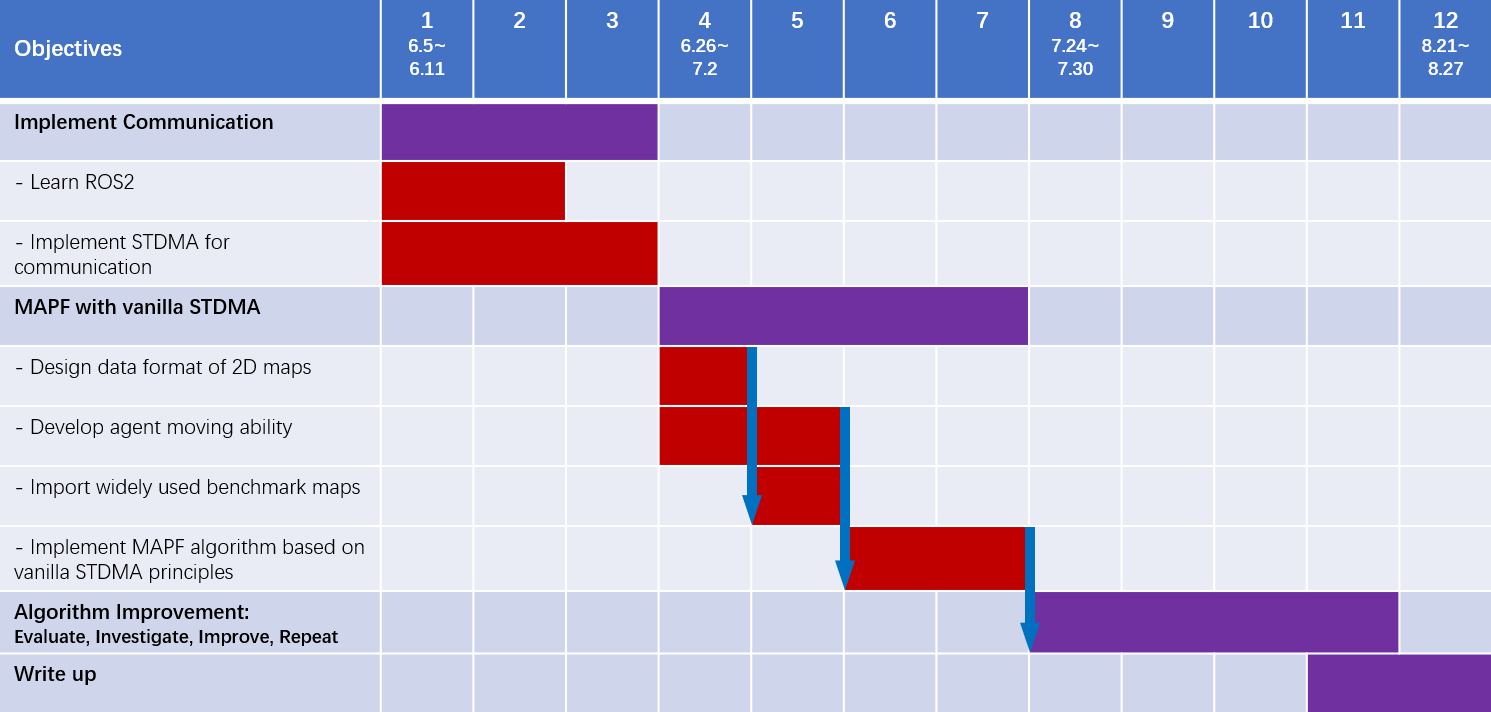
\includegraphics[width=1.1\textwidth]{Gannt Chart.png}}
    \caption{Project Gantt Chart.}
    \label{GanntChart}
\end{figure} 

Note: The actual available time is slightly longer than 12 weeks.

\patchcmd{\thebibliography}{\section*{\refname}}{}{}{}

\section{References}

\bibliographystyle{unsrt}
\bibliography{sample}

\end{document}